%% Patent Application: Apparatus for Frequency-Selective Protein Folding Modulation
%% with Temperature Compensation and Isotope-Shift Capability
%% Inventor: Jonathan Washburn
%% Contact: washburn.jonathan@gmail.com
%% Filing Date: January 2026

\documentclass[12pt,letterpaper]{article}

\usepackage[margin=1in]{geometry}
\usepackage{amsmath,amssymb,amsfonts}
\usepackage{graphicx}
\usepackage{tikz}
\usetikzlibrary{shapes,arrows,positioning,calc,patterns,decorations.pathmorphing}
\usepackage{booktabs}
\usepackage{array}
\usepackage{enumitem}
\usepackage{fancyhdr}
\usepackage{xcolor}
\usepackage{hyperref}
\usepackage{setspace}

% Patent-style formatting
\setlength{\parindent}{0.5in}
\setlength{\parskip}{0.5em}
\onehalfspacing

% Header
\pagestyle{fancy}
\fancyhf{}
\rhead{Patent Application}
\lhead{Washburn}
\rfoot{Page \thepage}

\hypersetup{
    colorlinks=true,
    linkcolor=blue,
    urlcolor=blue,
    citecolor=blue
}

% Custom colors
\definecolor{microwave}{RGB}{255,100,100}
\definecolor{cooling}{RGB}{100,100,255}
\definecolor{sensor}{RGB}{100,200,100}
\definecolor{chamber}{RGB}{200,200,200}

\begin{document}

%% ============================================================================
%%                              TITLE PAGE
%% ============================================================================

\begin{center}
\vspace*{0.8in}

{\LARGE \textbf{PATENT APPLICATION}}

\vspace{0.4in}

{\Large \textbf{APPARATUS FOR FREQUENCY-SELECTIVE}}

{\Large \textbf{PROTEIN FOLDING MODULATION WITH}}

{\Large \textbf{TEMPERATURE COMPENSATION AND}}

{\Large \textbf{ISOTOPE-SHIFT CAPABILITY}}

\vspace{0.8in}

\textbf{PROVISIONAL PATENT APPLICATION}

\vspace{0.5in}

\begin{tabular}{ll}
\textbf{Inventor:} & Jonathan Washburn \\
\textbf{Email:} & washburn.jonathan@gmail.com \\
\textbf{Filing Date:} & January 17, 2026 \\
\textbf{Application Type:} & Utility Patent (Provisional) \\
\textbf{Related Application:} & Patent 001 (Method Patent) \\
\end{tabular}

\vspace{0.8in}

\textit{An apparatus for precision microwave irradiation of protein samples at the resonant jamming frequency ($\sim$14.65 GHz), featuring active temperature compensation to distinguish resonant effects from thermal heating, and automatic isotope-shift frequency scaling for D$_2$O verification experiments.}

\vfill

\textbf{CONFIDENTIAL --- PATENT PENDING}

\end{center}

\newpage

%% ============================================================================
%%                         TABLE OF CONTENTS
%% ============================================================================

\tableofcontents
\newpage

%% ============================================================================
%%                              ABSTRACT
%% ============================================================================

\section*{ABSTRACT OF THE DISCLOSURE}
\addcontentsline{toc}{section}{ABSTRACT OF THE DISCLOSURE}

An apparatus for modulating protein folding rates through precision microwave irradiation at resonant frequencies. The apparatus comprises: (a) a frequency-agile microwave source tunable across 8--20 GHz with resolution of 0.001 GHz; (b) a thermally-controlled sample chamber with active temperature regulation to $\pm$0.05$^\circ$C; (c) a real-time folding detection system; (d) a closed-loop feedback controller that maintains isothermal conditions during irradiation; and (e) an isotope-mode controller that automatically scales the operating frequency by factor $1/\sqrt{2}$ for D$_2$O experiments. The apparatus enables unambiguous discrimination between resonant and thermal effects on protein folding by maintaining constant sample temperature while varying irradiation frequency. Key innovations include: temperature-compensated power modulation to eliminate thermal artifacts; dual-frequency operation for simultaneous H$_2$O/D$_2$O comparison; pulsed irradiation modes for intermediate trapping; and integration with spectroscopic detection systems. The apparatus implements the resonant protein folding modulation method derived from Recognition Science, targeting the molecular gate timescale $\tau_{19} \approx 68$ ps corresponding to a jamming frequency of approximately 14.65 GHz.

\vspace{1em}
\noindent\textbf{Keywords:} microwave apparatus, protein folding, temperature compensation, isotope shift, frequency-selective irradiation, molecular gate, resonant modulation

\newpage

%% ============================================================================
%%                      BACKGROUND OF THE INVENTION
%% ============================================================================

\section{BACKGROUND OF THE INVENTION}

\subsection{Field of the Invention}

The present invention relates generally to apparatus for studying and controlling protein folding, and more specifically to precision microwave irradiation systems with temperature compensation and isotope-shift capability for resonant modulation of protein conformational dynamics.

\subsection{Description of Related Art}

\subsubsection{Existing Microwave Irradiation Systems}

Prior art microwave systems used in biochemistry include:

\begin{enumerate}[label=(\alph*)]
\item \textbf{Domestic/industrial microwave ovens:} Operating at 2.45 GHz (ISM band), these devices provide bulk heating with no frequency selectivity. Temperature control is typically $\pm$5$^\circ$C at best, far too imprecise for distinguishing resonant from thermal effects.

\item \textbf{Microwave synthesizers:} Laboratory microwave reactors for chemical synthesis (e.g., CEM Discover, Biotage Initiator) operate at 2.45 GHz with improved temperature monitoring but still rely on thermal mechanisms. Frequency is fixed.

\item \textbf{Dielectric spectroscopy systems:} Broadband systems for measuring dielectric properties can sweep from MHz to THz but are designed for measurement, not controlled irradiation. Power levels are typically too low for biological effects.

\item \textbf{NMR/MRI systems:} While highly precise, these operate at much lower frequencies (100--900 MHz for NMR, 60--400 MHz for MRI) and are designed for spectroscopy/imaging, not protein folding modulation.

\item \textbf{Terahertz sources:} THz systems (0.1--10 THz) probe higher-frequency molecular vibrations but are outside the molecular gate frequency range relevant to protein folding.
\end{enumerate}

\subsubsection{Limitations of Prior Art Apparatus}

\begin{table}[h]
\centering
\begin{tabular}{p{0.25\textwidth}p{0.65\textwidth}}
\toprule
\textbf{Limitation} & \textbf{Description} \\
\midrule
Wrong frequency range & Prior systems operate at 2.45 GHz or in THz range; none target 12--17 GHz \\
\addlinespace
Poor temperature control & $\pm$1--5$^\circ$C typical; insufficient to distinguish resonant from thermal effects \\
\addlinespace
No isotope mode & No systems provide automatic frequency scaling for D$_2$O experiments \\
\addlinespace
No feedback control & Open-loop operation leads to uncontrolled sample heating \\
\addlinespace
No folding detection & Separate apparatus required for monitoring; no integrated real-time detection \\
\addlinespace
No pulsed operation & Continuous-wave only; cannot trap folding intermediates \\
\bottomrule
\end{tabular}
\caption{Limitations of prior art microwave apparatus}
\end{table}

\subsubsection{The Need for Precision Apparatus}

The method of resonant protein folding modulation (described in related Patent Application 001) requires apparatus with specific capabilities not available in any prior art system:

\begin{enumerate}[label=(\arabic*)]
\item \textbf{Frequency precision:} The jamming frequency at 14.65 GHz must be set with precision of at least 0.01 GHz to ensure resonance.

\item \textbf{Temperature stability:} To distinguish resonant from thermal effects, sample temperature must be maintained within $\pm$0.1$^\circ$C despite microwave absorption.

\item \textbf{Isotope-shift capability:} For verification experiments, the frequency must be scalable by exactly $1/\sqrt{2}$ for D$_2$O operation.

\item \textbf{Real-time monitoring:} Protein folding state must be monitored during irradiation to detect resonant effects.

\item \textbf{Feedback control:} Closed-loop control is required to maintain isothermal conditions while varying frequency.
\end{enumerate}

\subsection{Objects of the Invention}

It is an object of the present invention to provide apparatus that:

\begin{enumerate}[label=(\arabic*)]
\item Generates precision microwave radiation at frequencies in the 8--20 GHz range with resolution of 0.001 GHz;
\item Maintains sample temperature to within $\pm$0.1$^\circ$C during irradiation;
\item Provides automatic frequency scaling for isotope-shift experiments;
\item Integrates real-time protein folding detection;
\item Implements closed-loop feedback for isothermal operation;
\item Supports pulsed irradiation for intermediate trapping experiments.
\end{enumerate}

\newpage

%% ============================================================================
%%                      SUMMARY OF THE INVENTION
%% ============================================================================

\section{SUMMARY OF THE INVENTION}

\subsection{General Statement of the Invention}

The present invention provides an integrated apparatus for resonant protein folding modulation comprising:

\begin{enumerate}[label=(\alph*)]
\item A frequency-agile microwave source with continuous tunability from 8 to 20 GHz;
\item A precision sample chamber with microwave-transparent windows and integrated temperature control;
\item A multi-modal folding detection system;
\item A closed-loop feedback controller for isothermal operation;
\item An isotope-mode controller for automatic frequency scaling;
\item A pulsed irradiation controller for intermediate trapping.
\end{enumerate}

\subsection{Key Technical Innovations}

\subsubsection{Temperature-Compensated Power Modulation}

The apparatus implements a novel temperature-compensated power modulation (TCPM) algorithm:

\begin{equation}
P(t) = P_{\text{target}} \times \left[1 - k_p (T(t) - T_{\text{set}}) - k_i \int_0^t (T(s) - T_{\text{set}}) \, ds\right]
\label{eq:tcpm}
\end{equation}

where $P(t)$ is the instantaneous power, $T(t)$ is the measured temperature, $T_{\text{set}}$ is the target temperature, and $k_p$, $k_i$ are proportional and integral gain constants. This algorithm adjusts microwave power in real-time to maintain constant sample temperature despite varying absorption.

\subsubsection{Isotope-Shift Frequency Scaling}

The apparatus includes a dedicated isotope-mode controller that implements:

\begin{equation}
f_{\text{D}_2\text{O}} = \frac{f_{\text{H}_2\text{O}}}{\sqrt{2}} \approx 0.7071 \times f_{\text{H}_2\text{O}}
\label{eq:isotope_scale}
\end{equation}

When isotope mode is activated, the controller automatically:
\begin{enumerate}[label=(\roman*)]
\item Scales the operating frequency by factor $1/\sqrt{2}$;
\item Adjusts power levels to account for different D$_2$O dielectric properties;
\item Modifies temperature control parameters for D$_2$O thermal characteristics.
\end{enumerate}

\subsubsection{Dual-Chamber Configuration}

An optional dual-chamber configuration allows simultaneous irradiation of H$_2$O and D$_2$O samples at their respective resonant frequencies, enabling real-time comparison under identical conditions.

\subsection{Functional Block Diagram}

The apparatus comprises the following functional blocks:

\begin{figure}[h]
\centering
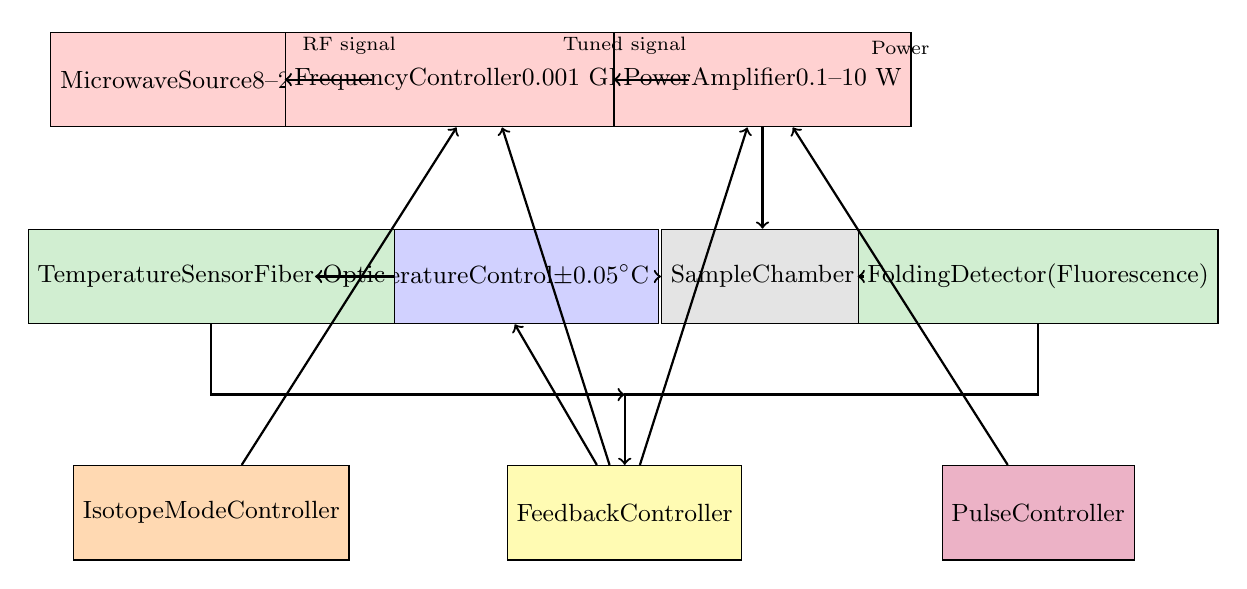
\begin{tikzpicture}[
    block/.style={rectangle, draw, minimum width=2.2cm, minimum height=1.2cm, text centered, font=\small},
    smallblock/.style={rectangle, draw, minimum width=1.8cm, minimum height=0.8cm, text centered, font=\scriptsize},
    arrow/.style={->, thick},
    dashedarrow/.style={->, thick, dashed}
]
    % Main blocks
    \node[block, fill=microwave!30] (source) at (0,4) {Microwave\\Source\\8--20 GHz};
    \node[block, fill=microwave!30] (freq) at (3.5,4) {Frequency\\Controller\\0.001 GHz res};
    \node[block, fill=microwave!30] (power) at (7,4) {Power\\Amplifier\\0.1--10 W};
    
    \node[block, fill=chamber!50] (chamber) at (7,1.5) {Sample\\Chamber};
    \node[block, fill=cooling!30] (temp) at (3.5,1.5) {Temperature\\Control\\$\pm$0.05$^\circ$C};
    \node[block, fill=sensor!30] (sensor) at (0,1.5) {Temperature\\Sensor\\Fiber Optic};
    
    \node[block, fill=sensor!30] (detect) at (10.5,1.5) {Folding\\Detector\\(Fluorescence)};
    
    \node[block, fill=yellow!30] (feedback) at (5.25,-1.5) {Feedback\\Controller};
    \node[block, fill=orange!30] (isotope) at (0,-1.5) {Isotope\\Mode\\Controller};
    \node[block, fill=purple!30] (pulse) at (10.5,-1.5) {Pulse\\Controller};
    
    % Arrows
    \draw[arrow] (source) -- (freq);
    \draw[arrow] (freq) -- (power);
    \draw[arrow] (power) -- (chamber);
    \draw[arrow] (chamber) -- (detect);
    \draw[arrow] (temp) -- (chamber);
    \draw[arrow] (sensor) -- (temp);
    
    \draw[arrow] (detect) -- (10.5,0) -- (5.25,0) -- (feedback);
    \draw[arrow] (sensor) -- (0,0) -- (5.25,0);
    
    \draw[arrow] (feedback) -- (freq);
    \draw[arrow] (feedback) -- (power);
    \draw[arrow] (feedback) -- (temp);
    
    \draw[arrow] (isotope) -- (freq);
    \draw[arrow] (pulse) -- (power);
    
    % Labels
    \node[above, font=\scriptsize] at (1.75,4.2) {RF signal};
    \node[above, font=\scriptsize] at (5.25,4.2) {Tuned signal};
    \node[above, font=\scriptsize] at (8.75,4.2) {Power};
    
\end{tikzpicture}
\caption{Functional block diagram of the apparatus}
\label{fig:block_diagram}
\end{figure}

\newpage

%% ============================================================================
%%                    BRIEF DESCRIPTION OF DRAWINGS
%% ============================================================================

\section{BRIEF DESCRIPTION OF DRAWINGS}

\subsection*{Figure 1: Functional Block Diagram}
A block diagram showing the interconnection of the major functional components: microwave source, frequency controller, power amplifier, sample chamber, temperature control system, folding detector, feedback controller, isotope mode controller, and pulse controller.

\subsection*{Figure 2: Sample Chamber Cross-Section}
A cross-sectional view of the sample chamber showing: microwave waveguide, quartz sample holder, Peltier cooling elements, fiber-optic temperature sensor, fluorescence excitation/detection optics, and thermal insulation.

\subsection*{Figure 3: Temperature Control Loop}
A control system diagram showing the feedback loop for maintaining isothermal conditions during microwave irradiation.

\subsection*{Figure 4: Isotope Mode Operation}
A diagram illustrating the frequency scaling for H$_2$O vs.\ D$_2$O operation.

\subsection*{Figure 5: Pulse Timing Diagrams}
Timing diagrams showing various pulse modes for intermediate trapping experiments.

\subsection*{Figure 6: Dual-Chamber Configuration}
A diagram of the optional dual-chamber system for simultaneous H$_2$O/D$_2$O comparison.

\newpage

%% ============================================================================
%%                      DETAILED DESCRIPTION
%% ============================================================================

\section{DETAILED DESCRIPTION OF THE PREFERRED EMBODIMENTS}

\subsection{Microwave Source Subsystem}

\subsubsection{Frequency-Agile Source}

The microwave source subsystem comprises a frequency-agile signal generator with the following specifications:

\begin{table}[h]
\centering
\begin{tabular}{ll}
\toprule
\textbf{Parameter} & \textbf{Specification} \\
\midrule
Frequency range & 8--20 GHz (continuous) \\
Frequency resolution & 0.001 GHz (1 MHz) \\
Frequency accuracy & $\pm$0.0001 GHz ($\pm$100 kHz) \\
Frequency stability & $\pm$1 ppm over operating temperature \\
Phase noise & $<$ --100 dBc/Hz at 10 kHz offset \\
Switching time & $<$ 1 ms \\
Output power (pre-amp) & 0 to +10 dBm \\
\bottomrule
\end{tabular}
\caption{Microwave source specifications}
\end{table}

The source is based on a phase-locked loop (PLL) synthesizer architecture with a low-noise reference oscillator. Preferred implementations include:

\begin{enumerate}[label=(\roman*)]
\item Yttrium iron garnet (YIG) oscillator with PLL control;
\item Direct digital synthesis (DDS) with frequency multiplication;
\item Voltage-controlled oscillator (VCO) bank with PLL.
\end{enumerate}

\subsubsection{Power Amplifier}

The power amplifier provides the following characteristics:

\begin{table}[h]
\centering
\begin{tabular}{ll}
\toprule
\textbf{Parameter} & \textbf{Specification} \\
\midrule
Frequency range & 8--20 GHz \\
Output power & 0.1 to 10 W (continuously adjustable) \\
Power resolution & 0.01 W \\
Power accuracy & $\pm$0.1 W or $\pm$5\%, whichever is greater \\
Harmonic suppression & $>$ 30 dB \\
Modulation bandwidth & DC to 10 MHz (for pulsed operation) \\
\bottomrule
\end{tabular}
\caption{Power amplifier specifications}
\end{table}

Preferred implementations use traveling-wave tube (TWT) amplifiers or solid-state GaN power amplifiers.

\subsubsection{Frequency Controller}

The frequency controller implements the following functions:

\begin{enumerate}[label=(\arabic*)]
\item \textbf{Manual frequency setting:} Direct entry of target frequency via digital interface.

\item \textbf{Frequency sweep:} Programmable frequency sweeps for resonance mapping:
\begin{equation}
f(t) = f_{\text{start}} + \frac{f_{\text{stop}} - f_{\text{start}}}{t_{\text{sweep}}} \times t
\end{equation}

\item \textbf{Isotope scaling:} Automatic application of $1/\sqrt{2}$ factor when isotope mode is active.

\item \textbf{Feedback adjustment:} Fine frequency adjustment based on feedback controller input.
\end{enumerate}

\subsection{Sample Chamber Subsystem}

\subsubsection{Chamber Design}

The sample chamber is designed to:

\begin{enumerate}[label=(\alph*)]
\item Efficiently couple microwave energy into the sample;
\item Provide optical access for fluorescence detection;
\item Enable precise temperature control;
\item Accommodate both H$_2$O and D$_2$O samples;
\item Minimize sample volume while maintaining uniform irradiation.
\end{enumerate}

\begin{figure}[h]
\centering
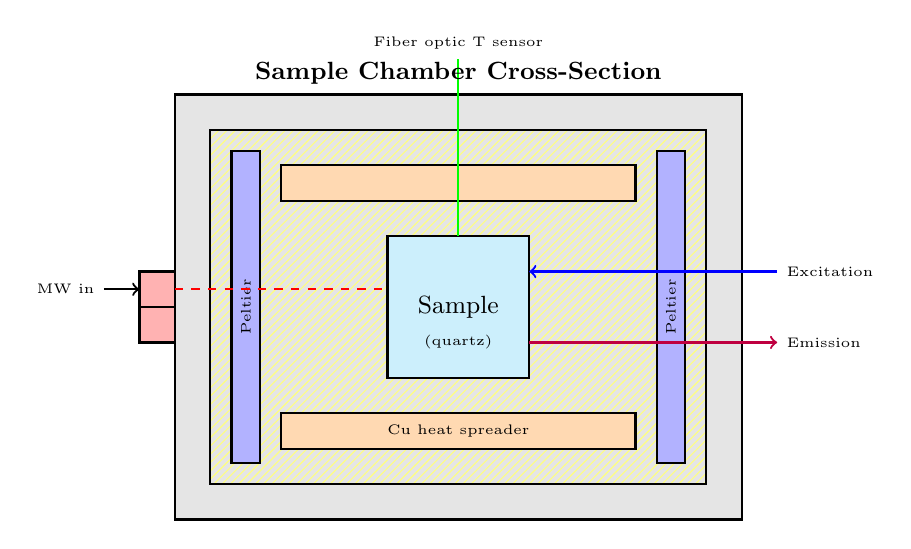
\begin{tikzpicture}[scale=0.9]
    % Outer housing
    \draw[thick, fill=gray!20] (-4,-3) rectangle (4,3);
    
    % Thermal insulation
    \draw[thick, fill=yellow!20, pattern=north east lines, pattern color=yellow!50] (-3.5,-2.5) rectangle (3.5,2.5);
    
    % Peltier elements
    \draw[thick, fill=blue!30] (-3.2,-2.2) rectangle (-2.8,2.2);
    \draw[thick, fill=blue!30] (2.8,-2.2) rectangle (3.2,2.2);
    \node[font=\tiny, rotate=90] at (-3,0) {Peltier};
    \node[font=\tiny, rotate=90] at (3,0) {Peltier};
    
    % Copper heat spreader
    \draw[thick, fill=orange!30] (-2.5,-2) rectangle (2.5,-1.5);
    \draw[thick, fill=orange!30] (-2.5,1.5) rectangle (2.5,2);
    \node[font=\tiny] at (0,-1.75) {Cu heat spreader};
    
    % Sample holder (quartz)
    \draw[thick, fill=cyan!20] (-1,-1) rectangle (1,1);
    \node[font=\small] at (0,0) {Sample};
    \node[font=\tiny] at (0,-0.5) {(quartz)};
    
    % Waveguide input
    \draw[thick, fill=red!30] (-4.5,0) rectangle (-4,-0.5);
    \draw[thick, fill=red!30] (-4.5,0.5) rectangle (-4,0);
    \draw[thick, ->] (-5,0.25) -- (-4.5,0.25);
    \node[font=\tiny, left] at (-5,0.25) {MW in};
    
    % Waveguide coupling
    \draw[thick, dashed, red] (-4,0.25) -- (-1,0.25);
    
    % Fiber optic temperature sensor
    \draw[thick, green] (0,1) -- (0,3.5);
    \node[font=\tiny, above] at (0,3.5) {Fiber optic T sensor};
    
    % Fluorescence optics
    \draw[thick, blue, ->] (4.5,0.5) -- (1,0.5);
    \node[font=\tiny, right] at (4.5,0.5) {Excitation};
    \draw[thick, purple, <-] (4.5,-0.5) -- (1,-0.5);
    \node[font=\tiny, right] at (4.5,-0.5) {Emission};
    
    % Labels
    \node[font=\small, above] at (0,3) {\textbf{Sample Chamber Cross-Section}};
    
\end{tikzpicture}
\caption{Cross-sectional view of the sample chamber showing thermal management and optical access}
\label{fig:chamber}
\end{figure}

\subsubsection{Sample Holder}

The sample holder is constructed from high-purity fused quartz (SiO$_2$) with the following properties:

\begin{table}[h]
\centering
\begin{tabular}{ll}
\toprule
\textbf{Property} & \textbf{Value} \\
\midrule
Material & Fused quartz (Suprasil or equivalent) \\
Dielectric constant (10--20 GHz) & $\sim$3.8 \\
Loss tangent (10--20 GHz) & $<$ 0.0001 \\
Optical transmission & $>$ 90\% (250--700 nm) \\
Thermal conductivity & $\sim$1.4 W/(m$\cdot$K) \\
Sample volume & 50--500 $\mu$L (configurable) \\
Wall thickness & 0.5--1.0 mm \\
\bottomrule
\end{tabular}
\caption{Sample holder specifications}
\end{table}

Alternative materials include:
\begin{enumerate}[label=(\roman*)]
\item Sapphire (Al$_2$O$_3$): Higher thermal conductivity but higher cost;
\item Borosilicate glass: Lower cost but higher microwave losses;
\item PTFE (Teflon): Low dielectric loss but poor optical properties.
\end{enumerate}

\subsubsection{Microwave Coupling}

Microwave energy is coupled into the sample chamber via:

\begin{enumerate}[label=(\arabic*)]
\item \textbf{Rectangular waveguide:} WR-62 (12.4--18 GHz) or WR-42 (18--26.5 GHz) with tapered transition for broadband operation.

\item \textbf{Coaxial-to-waveguide adapter:} For connecting to the power amplifier output.

\item \textbf{Impedance matching:} Tunable iris or stub matching network to optimize power transfer to the sample.

\item \textbf{Field uniformity:} Cavity design or mode stirrer to ensure uniform field distribution across the sample volume.
\end{enumerate}

\subsection{Temperature Control Subsystem}

\subsubsection{Design Requirements}

Temperature control is critical for distinguishing resonant from thermal effects. The subsystem must:

\begin{enumerate}[label=(\alph*)]
\item Maintain sample temperature to $\pm$0.05$^\circ$C (goal) or $\pm$0.1$^\circ$C (minimum);
\item Respond to power absorption within 100 ms;
\item Operate over temperature range of 4--50$^\circ$C;
\item Function with both H$_2$O and D$_2$O samples.
\end{enumerate}

\subsubsection{Temperature Sensor}

The preferred temperature sensor is a fiber-optic fluorescence-based thermometer:

\begin{table}[h]
\centering
\begin{tabular}{ll}
\toprule
\textbf{Parameter} & \textbf{Specification} \\
\midrule
Type & Fluorescence decay (GaAs or similar) \\
Resolution & 0.01$^\circ$C \\
Accuracy & $\pm$0.05$^\circ$C \\
Response time & $<$ 50 ms \\
Immunity to RF/microwave & Complete (no metallic components) \\
Operating range & --40 to +200$^\circ$C \\
Probe diameter & $<$ 1 mm \\
\bottomrule
\end{tabular}
\caption{Temperature sensor specifications}
\end{table}

The fiber-optic sensor is immune to electromagnetic interference from the microwave field, unlike thermocouples or RTDs.

\subsubsection{Thermal Management}

Active temperature control is provided by:

\begin{enumerate}[label=(\arabic*)]
\item \textbf{Peltier (thermoelectric) modules:} Bi$_2$Te$_3$-based modules provide heating and cooling capacity of 10--50 W.

\item \textbf{Heat spreaders:} Copper plates with high thermal conductivity ($\sim$400 W/(m$\cdot$K)) distribute heat evenly.

\item \textbf{Heat sink/fan:} External heat rejection for Peltier hot side.

\item \textbf{Thermal insulation:} Aerogel or vacuum insulation to minimize heat exchange with environment.
\end{enumerate}

\subsubsection{Control Algorithm}

The temperature control implements a PID (proportional-integral-derivative) controller with feedforward compensation:

\begin{equation}
Q(t) = K_p e(t) + K_i \int_0^t e(\tau) \, d\tau + K_d \frac{de(t)}{dt} - K_{ff} P_{\text{MW}}(t)
\label{eq:pid}
\end{equation}

where:
\begin{itemize}
\item $Q(t)$ = Peltier heating/cooling power
\item $e(t) = T_{\text{set}} - T(t)$ = temperature error
\item $K_p$, $K_i$, $K_d$ = PID gains
\item $K_{ff}$ = feedforward gain
\item $P_{\text{MW}}(t)$ = microwave power
\end{itemize}

The feedforward term ($K_{ff} P_{\text{MW}}$) anticipates sample heating due to microwave absorption and preemptively activates cooling, reducing temperature excursions.

\begin{figure}[h]
\centering
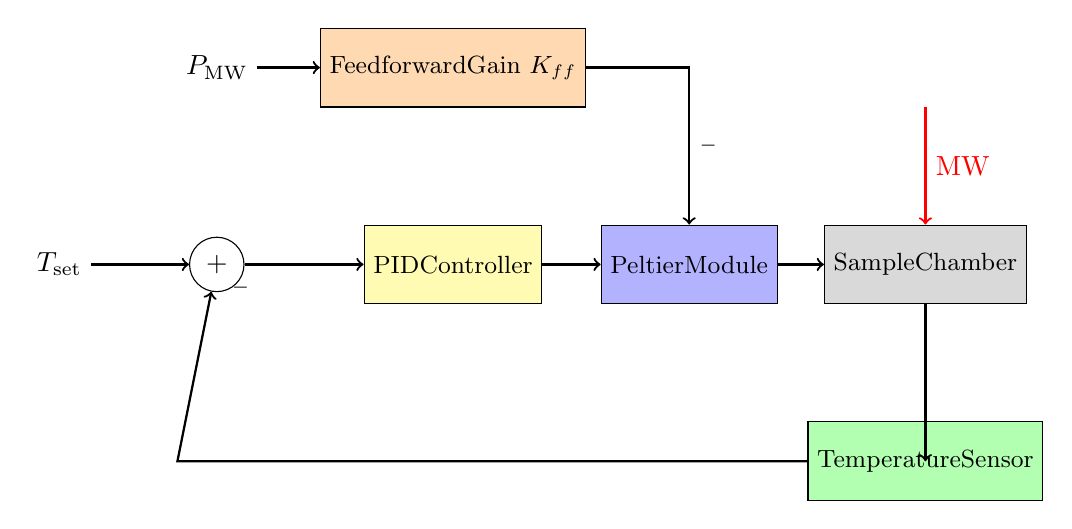
\begin{tikzpicture}[
    block/.style={rectangle, draw, minimum width=1.8cm, minimum height=1cm, text centered, font=\small},
    sum/.style={circle, draw, minimum size=0.6cm},
    arrow/.style={->, thick}
]
    % Setpoint
    \node (setpoint) at (-2,0) {$T_{\text{set}}$};
    
    % Summing junction
    \node[sum] (sum) at (0,0) {$+$};
    \node at (0.3,-0.3) {\scriptsize $-$};
    
    % PID controller
    \node[block, fill=yellow!30] (pid) at (3,0) {PID\\Controller};
    
    % Peltier
    \node[block, fill=blue!30] (peltier) at (6,0) {Peltier\\Module};
    
    % Sample
    \node[block, fill=gray!30] (sample) at (9,0) {Sample\\Chamber};
    
    % Sensor
    \node[block, fill=green!30] (sensor) at (9,-2.5) {Temperature\\Sensor};
    
    % Feedforward
    \node[block, fill=orange!30] (ff) at (3,2.5) {Feedforward\\Gain $K_{ff}$};
    \node (mw) at (0,2.5) {$P_{\text{MW}}$};
    
    % Microwave input
    \draw[arrow, red, thick] (9,2) -- node[right] {MW} (sample);
    
    % Connections
    \draw[arrow] (setpoint) -- (sum);
    \draw[arrow] (sum) -- (pid);
    \draw[arrow] (pid) -- (peltier);
    \draw[arrow] (peltier) -- (sample);
    \draw[arrow] (sample) -- (9,-2.5);
    \draw[arrow] (sensor) -- (-0.5,-2.5) -- (sum);
    
    \draw[arrow] (mw) -- (ff);
    \draw[arrow] (ff) -- (6,2.5) -- node[right] {\scriptsize $-$} (peltier);
    
\end{tikzpicture}
\caption{Temperature control loop with feedforward compensation for microwave heating}
\label{fig:temp_control}
\end{figure}

\subsection{Folding Detection Subsystem}

\subsubsection{Detection Modalities}

The apparatus supports multiple detection modalities:

\begin{enumerate}[label=(\arabic*)]
\item \textbf{Intrinsic tryptophan fluorescence:}
\begin{itemize}
\item Excitation: 280--295 nm (UV LED or laser)
\item Emission: 320--360 nm
\item Sensitivity: Detects tertiary structure changes
\end{itemize}

\item \textbf{FRET (Förster Resonance Energy Transfer):}
\begin{itemize}
\item Requires labeled protein (donor/acceptor pair)
\item Measures intramolecular distances
\item High sensitivity to folding state
\end{itemize}

\item \textbf{Circular dichroism (CD):}
\begin{itemize}
\item Far-UV (190--250 nm) for secondary structure
\item Near-UV (250--320 nm) for tertiary structure
\item Requires external CD spectrometer integration
\end{itemize}

\item \textbf{Dynamic light scattering (DLS):}
\begin{itemize}
\item Measures hydrodynamic radius
\item Detects aggregation
\item Requires external DLS module
\end{itemize}
\end{enumerate}

\subsubsection{Preferred Implementation: Fluorescence Detection}

The preferred embodiment uses intrinsic tryptophan fluorescence with:

\begin{table}[h]
\centering
\begin{tabular}{ll}
\toprule
\textbf{Component} & \textbf{Specification} \\
\midrule
Excitation source & 280 nm LED or 266 nm laser \\
Excitation bandwidth & 10 nm (bandpass filter) \\
Excitation power & 1--10 mW \\
Emission filter & 340 $\pm$ 20 nm bandpass \\
Detector & Photomultiplier tube (PMT) or Si APD \\
Sampling rate & 10--1000 Hz \\
Dynamic range & 4 decades \\
\bottomrule
\end{tabular}
\caption{Fluorescence detection specifications}
\end{table}

\subsection{Feedback Controller Subsystem}

\subsubsection{Controller Architecture}

The feedback controller is a digital signal processor (DSP) or field-programmable gate array (FPGA) implementing:

\begin{enumerate}[label=(\arabic*)]
\item Temperature feedback loop (Equation~\ref{eq:pid});
\item Power modulation for isothermal operation (Equation~\ref{eq:tcpm});
\item Frequency optimization based on folding signal;
\item Safety interlocks (over-temperature, over-power).
\end{enumerate}

\subsubsection{Isothermal Operation Mode}

In isothermal mode, the controller maintains constant sample temperature while irradiating at different frequencies. This is achieved by:

\begin{enumerate}[label=(\alph*)]
\item Setting target temperature $T_{\text{set}}$;
\item Monitoring temperature continuously ($>$ 10 Hz);
\item Adjusting Peltier power via PID + feedforward;
\item If temperature deviates $>$ 0.2$^\circ$C, reducing microwave power;
\item Logging all parameters for post-experiment analysis.
\end{enumerate}

\subsubsection{Resonance Search Mode}

In resonance search mode, the controller:

\begin{enumerate}[label=(\alph*)]
\item Sweeps frequency across a programmed range (e.g., 12--17 GHz);
\item Monitors folding signal at each frequency;
\item Identifies frequency of minimum folding rate (resonance);
\item Optionally performs fine sweep around identified minimum;
\item Reports resonance frequency and width.
\end{enumerate}

\subsection{Isotope Mode Controller}

\subsubsection{Frequency Scaling}

When operating with D$_2$O samples, the isotope mode controller:

\begin{enumerate}[label=(\arabic*)]
\item Receives notification of D$_2$O sample loading (manual or automatic detection);
\item Computes scaled frequency: $f_{\text{D}_2\text{O}} = f_{\text{H}_2\text{O}} / \sqrt{2}$;
\item Commands frequency controller to apply scaled frequency;
\item Adjusts power calibration for D$_2$O dielectric properties;
\item Modifies temperature control parameters for D$_2$O thermal properties.
\end{enumerate}

\subsubsection{Automatic Solvent Detection (Optional)}

An optional dielectric sensor can automatically detect the solvent:

\begin{itemize}
\item H$_2$O: $\varepsilon' \approx 80$ at low frequency, $\varepsilon' \approx 30$ at 15 GHz
\item D$_2$O: $\varepsilon' \approx 78$ at low frequency, slightly different dispersion
\end{itemize}

By measuring the dielectric constant at a reference frequency, the controller can automatically select the appropriate operating mode.

\begin{figure}[h]
\centering
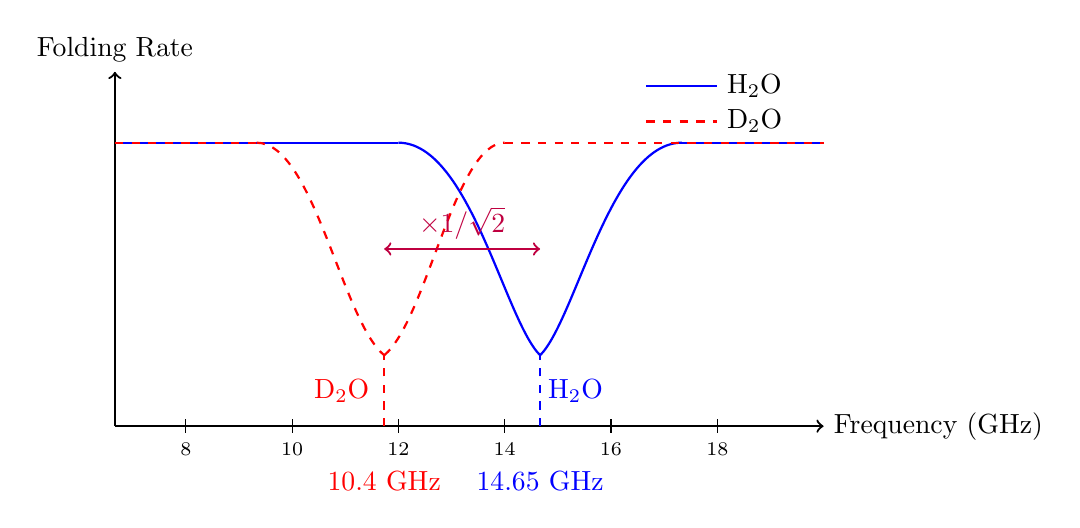
\begin{tikzpicture}[scale=0.9]
    % Axes
    \draw[thick,->] (0,0) -- (10,0) node[right] {Frequency (GHz)};
    \draw[thick,->] (0,0) -- (0,5) node[above] {Folding Rate};
    
    % Axis labels
    \foreach \x/\label in {1/8, 2.5/10, 4/12, 5.5/14, 7/16, 8.5/18} {
        \draw (\x,0.1) -- (\x,-0.1) node[below] {\scriptsize \label};
    }
    
    % H2O curve
    \draw[thick, blue] (0,4) -- (4,4);
    \draw[thick, blue] (4,4) .. controls (5,4) and (5.5,1.5) .. (6,1);
    \draw[thick, blue] (6,1) .. controls (6.5,1.5) and (7,4) .. (8,4);
    \draw[thick, blue] (8,4) -- (10,4);
    
    % D2O curve
    \draw[thick, red, dashed] (0,4) -- (2,4);
    \draw[thick, red, dashed] (2,4) .. controls (2.8,4) and (3.2,1.5) .. (3.8,1);
    \draw[thick, red, dashed] (3.8,1) .. controls (4.4,1.5) and (4.8,4) .. (5.5,4);
    \draw[thick, red, dashed] (5.5,4) -- (10,4);
    
    % Markers
    \draw[blue, thick, dashed] (6,0) -- (6,1);
    \node[blue, below] at (6,-0.5) {14.65 GHz};
    \node[blue] at (6.5,0.5) {H$_2$O};
    
    \draw[red, thick, dashed] (3.8,0) -- (3.8,1);
    \node[red, below] at (3.8,-0.5) {10.4 GHz};
    \node[red] at (3.2,0.5) {D$_2$O};
    
    % Arrow showing shift
    \draw[<->, thick, purple] (3.8,2.5) -- (6,2.5);
    \node[purple, above] at (4.9,2.5) {$\times 1/\sqrt{2}$};
    
    % Legend
    \draw[thick, blue] (7.5,4.8) -- (8.5,4.8);
    \node[right] at (8.5,4.8) {H$_2$O};
    \draw[thick, red, dashed] (7.5,4.3) -- (8.5,4.3);
    \node[right] at (8.5,4.3) {D$_2$O};
    
\end{tikzpicture}
\caption{Isotope mode frequency scaling: The resonance frequency shifts by factor $1/\sqrt{2}$ when H$_2$O is replaced by D$_2$O}
\label{fig:isotope_shift}
\end{figure}

\subsection{Pulse Controller Subsystem}

\subsubsection{Pulse Modes}

The apparatus supports several pulse modes for different applications:

\begin{enumerate}[label=(\arabic*)]
\item \textbf{Continuous wave (CW):} Constant power at fixed frequency.

\item \textbf{Gated CW:} Fixed frequency with programmable on/off duty cycle:
\begin{equation}
P(t) = \begin{cases} P_0 & \text{if } (t \mod T) < T_{\text{on}} \\ 0 & \text{otherwise} \end{cases}
\end{equation}

\item \textbf{Single pulse:} One-shot pulse with programmable duration (1 ns -- 1 s).

\item \textbf{Pulse train:} Multiple pulses with programmable spacing:
\begin{equation}
P(t) = P_0 \sum_{n=0}^{N-1} \Pi\left(\frac{t - nT_{\text{rep}} - T_{\text{pulse}}/2}{T_{\text{pulse}}}\right)
\end{equation}

\item \textbf{Chirped pulse:} Frequency swept during pulse for broadband excitation.
\end{enumerate}

\subsubsection{Timing Specifications}

\begin{table}[h]
\centering
\begin{tabular}{ll}
\toprule
\textbf{Parameter} & \textbf{Specification} \\
\midrule
Minimum pulse width & 1 ns \\
Maximum pulse width & Unlimited (CW) \\
Pulse width resolution & 1 ns \\
Rise/fall time & $<$ 5 ns \\
Repetition rate & DC to 10 MHz \\
Timing jitter & $<$ 100 ps RMS \\
Trigger delay & Programmable, 0--10 s \\
External trigger input & TTL/LVTTL, 50 $\Omega$ \\
\bottomrule
\end{tabular}
\caption{Pulse controller timing specifications}
\end{table}

\begin{figure}[h]
\centering
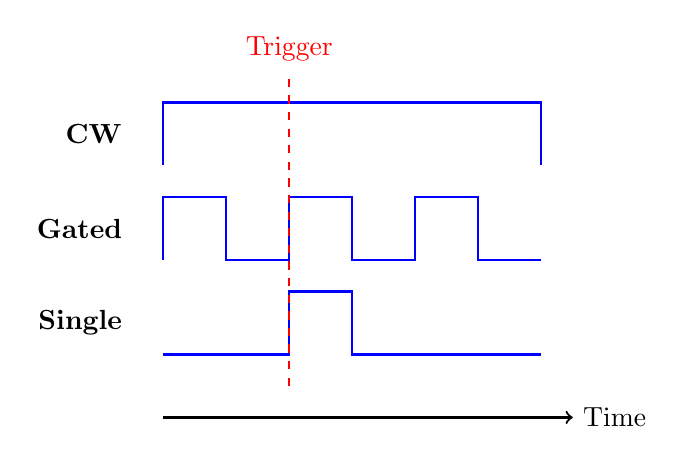
\begin{tikzpicture}[scale=0.8]
    % CW mode
    \node[left] at (-0.5,4) {\textbf{CW}};
    \draw[thick, blue] (0,3.5) -- (0,4.5) -- (6,4.5) -- (6,3.5);
    
    % Gated CW
    \node[left] at (-0.5,2.5) {\textbf{Gated}};
    \draw[thick, blue] (0,2) -- (0,3) -- (1,3) -- (1,2) -- (2,2) -- (2,3) -- (3,3) -- (3,2) -- (4,2) -- (4,3) -- (5,3) -- (5,2) -- (6,2);
    
    % Single pulse
    \node[left] at (-0.5,1) {\textbf{Single}};
    \draw[thick, blue] (0,0.5) -- (2,0.5) -- (2,1.5) -- (3,1.5) -- (3,0.5) -- (6,0.5);
    
    % Trigger
    \draw[thick, red, dashed] (2,0) -- (2,5);
    \node[red, above] at (2,5) {Trigger};
    
    % Time axis
    \draw[thick,->] (0,-0.5) -- (6.5,-0.5) node[right] {Time};
    
\end{tikzpicture}
\caption{Pulse timing diagrams: CW, gated, and single-pulse modes}
\label{fig:pulses}
\end{figure}

\subsection{Dual-Chamber Configuration (Optional)}

\subsubsection{Design Concept}

The optional dual-chamber configuration enables simultaneous irradiation of H$_2$O and D$_2$O samples under identical conditions:

\begin{figure}[h]
\centering
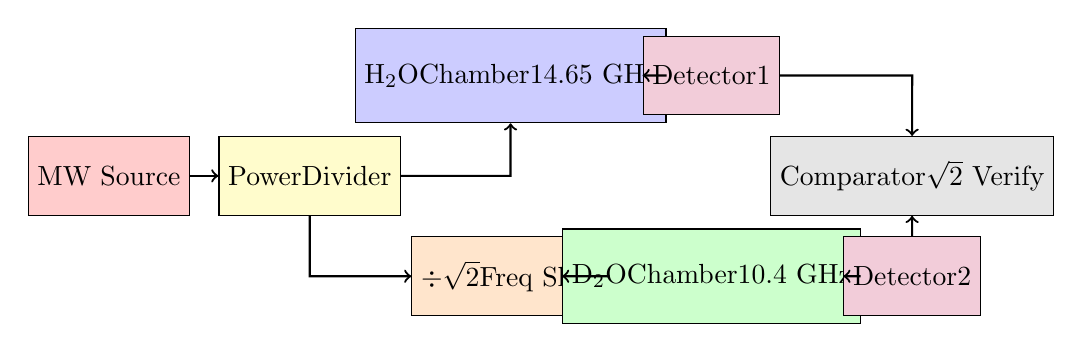
\begin{tikzpicture}[scale=0.85]
    % Source
    \node[rectangle, draw, fill=red!20, minimum width=2cm, minimum height=1cm] (source) at (0,0) {MW Source};
    
    % Power divider
    \node[rectangle, draw, fill=yellow!20, minimum width=1.5cm, minimum height=1cm] (divider) at (3,0) {Power\\Divider};
    
    % Frequency shifter
    \node[rectangle, draw, fill=orange!20, minimum width=1.5cm, minimum height=1cm] (shifter) at (6,-1.5) {$\div\sqrt{2}$\\Freq Shift};
    
    % Chambers
    \node[rectangle, draw, fill=blue!20, minimum width=2cm, minimum height=1.2cm] (h2o) at (6,1.5) {H$_2$O\\Chamber\\14.65 GHz};
    \node[rectangle, draw, fill=green!20, minimum width=2cm, minimum height=1.2cm] (d2o) at (9,-1.5) {D$_2$O\\Chamber\\10.4 GHz};
    
    % Detectors
    \node[rectangle, draw, fill=purple!20, minimum width=1.5cm, minimum height=1cm] (det1) at (9,1.5) {Detector\\1};
    \node[rectangle, draw, fill=purple!20, minimum width=1.5cm, minimum height=1cm] (det2) at (12,-1.5) {Detector\\2};
    
    % Comparator
    \node[rectangle, draw, fill=gray!20, minimum width=2cm, minimum height=1cm] (comp) at (12,0) {Comparator\\$\sqrt{2}$ Verify};
    
    % Arrows
    \draw[thick,->] (source) -- (divider);
    \draw[thick,->] (divider) -- (6,0) -- (h2o);
    \draw[thick,->] (divider) -- (3,-1.5) -- (shifter);
    \draw[thick,->] (shifter) -- (d2o);
    \draw[thick,->] (h2o) -- (det1);
    \draw[thick,->] (d2o) -- (det2);
    \draw[thick,->] (det1) -- (12,1.5) -- (comp);
    \draw[thick,->] (det2) -- (comp);
    
\end{tikzpicture}
\caption{Dual-chamber configuration for simultaneous H$_2$O/D$_2$O comparison}
\label{fig:dual_chamber}
\end{figure}

\subsubsection{Advantages}

The dual-chamber configuration provides:

\begin{enumerate}[label=(\alph*)]
\item Simultaneous measurement eliminates temporal drift;
\item Same microwave source ensures correlated frequency;
\item Direct comparison validates $\sqrt{2}$ isotope shift;
\item Rigorous control experiment in every run.
\end{enumerate}

\subsection{User Interface and Data Acquisition}

\subsubsection{Control Interface}

The apparatus is controlled via:

\begin{enumerate}[label=(\arabic*)]
\item \textbf{Local control panel:} Touchscreen display for basic operations.

\item \textbf{Computer interface:} USB, Ethernet, or GPIB connection to control computer running dedicated software.

\item \textbf{Scripting interface:} Python or MATLAB API for automated experiments.

\item \textbf{Remote access:} Web interface for remote monitoring and control.
\end{enumerate}

\subsubsection{Data Logging}

All parameters are logged with timestamps:

\begin{itemize}
\item Frequency (0.001 GHz resolution)
\item Power (0.01 W resolution)
\item Temperature (0.01$^\circ$C resolution)
\item Folding signal (16-bit ADC)
\item Pulse timing (1 ns resolution)
\item Isotope mode status
\end{itemize}

Data is stored in HDF5 format for efficient post-processing.

\subsection{Safety Features}

\subsubsection{Interlocks}

The apparatus includes safety interlocks:

\begin{enumerate}[label=(\arabic*)]
\item \textbf{Over-temperature:} Microwave power shuts off if $T > T_{\text{max}}$ (programmable, default 60$^\circ$C).

\item \textbf{Door interlock:} Power disabled when sample access door is open.

\item \textbf{Over-power:} Hardware limiter prevents $P > P_{\text{max}}$ (default 10 W).

\item \textbf{Thermal runaway:} Automatic shutdown if temperature rises $>$ 1$^\circ$C/s.

\item \textbf{Emergency stop:} Physical button immediately disables all power.
\end{enumerate}

\subsubsection{Shielding}

The apparatus is fully shielded to prevent microwave leakage:

\begin{itemize}
\item Enclosure: Aluminum or steel with conductive gaskets
\item Leakage specification: $<$ 1 mW/cm$^2$ at 5 cm from any surface (per IEEE C95.1)
\item Viewports: Conductive mesh (aperture $<$ $\lambda$/10)
\end{itemize}

\newpage

%% ============================================================================
%%                              CLAIMS
%% ============================================================================

\section{CLAIMS}

What is claimed is:

\subsection{Apparatus Claims}

\begin{enumerate}[label=\textbf{\arabic*.}]

\item An apparatus for modulating protein folding rate by resonant microwave irradiation, comprising:
\begin{enumerate}[label=(\alph*)}
\item a microwave source capable of generating electromagnetic radiation tunable in the frequency range of 8 to 20 GHz;
\item a frequency controller configured to set the frequency of said microwave source with a resolution of at least 0.01 GHz;
\item a sample chamber configured to hold a protein sample and to receive microwave radiation from said source;
\item a temperature sensor configured to measure the temperature of said sample;
\item a temperature control system configured to maintain the sample temperature within $\pm$0.1$^\circ$C of a target temperature;
\item a feedback controller configured to adjust at least one of microwave power and temperature control based on said temperature measurement; and
\item a folding detector configured to measure protein folding state in real time.
\end{enumerate}

\item The apparatus of claim 1, wherein the frequency controller is configured to set the frequency to approximately 14.65 $\pm$ 0.5 GHz for H$_2$O samples.

\item The apparatus of claim 1, further comprising an isotope mode controller configured to automatically scale the operating frequency by a factor of $1/\sqrt{2}$ when D$_2$O samples are used.

\item The apparatus of claim 3, wherein the isotope mode controller is configured to operate at approximately 10.4 $\pm$ 0.5 GHz for D$_2$O samples.

\item The apparatus of claim 1, wherein the temperature sensor comprises a fiber-optic fluorescence-based thermometer immune to electromagnetic interference from the microwave radiation.

\item The apparatus of claim 1, wherein the temperature control system comprises:
\begin{enumerate}[label=(\roman*)]
\item at least one Peltier thermoelectric module in thermal contact with said sample chamber;
\item a heat spreader configured to distribute thermal energy evenly across said sample chamber; and
\item a heat sink for rejecting heat from the hot side of said Peltier module.
\end{enumerate}

\item The apparatus of claim 1, wherein the feedback controller implements a PID control algorithm with feedforward compensation for microwave power absorption.

\item The apparatus of claim 7, wherein the feedforward compensation preemptively adjusts cooling in proportion to applied microwave power to minimize temperature excursions.

\item The apparatus of claim 1, wherein the sample chamber comprises a microwave-transparent sample holder made of fused quartz or sapphire.

\item The apparatus of claim 1, wherein the folding detector comprises a fluorescence detection system configured to measure intrinsic tryptophan fluorescence with excitation at 280--295 nm and emission detection at 320--360 nm.

\item The apparatus of claim 1, further comprising a power amplifier capable of output power from 0.1 to 10 W with power resolution of at least 0.01 W.

\item The apparatus of claim 1, further comprising a pulse controller configured to generate pulsed microwave radiation with pulse widths from 1 nanosecond to continuous wave.

\item The apparatus of claim 12, wherein the pulse controller is configured to generate:
\begin{enumerate}[label=(\roman*)]
\item single pulses with programmable duration;
\item pulse trains with programmable pulse spacing and number of pulses; and
\item gated continuous-wave operation with programmable duty cycle.
\end{enumerate}

\item The apparatus of claim 1, wherein the frequency controller is configured to perform frequency sweeps across a programmable frequency range for resonance mapping.

\item An apparatus for simultaneous comparison of protein folding in H$_2$O and D$_2$O samples, comprising:
\begin{enumerate}[label=(\alph*)]
\item a microwave source;
\item a power divider configured to split the output of said microwave source into two paths;
\item a first sample chamber for H$_2$O samples, irradiated at a first frequency $f_1$;
\item a frequency shifter configured to shift the frequency in the second path by a factor of $1/\sqrt{2}$;
\item a second sample chamber for D$_2$O samples, irradiated at a second frequency $f_2 = f_1/\sqrt{2}$;
\item a first folding detector associated with said first sample chamber;
\item a second folding detector associated with said second sample chamber; and
\item a comparator configured to compare folding rates in said first and second sample chambers.
\end{enumerate}

\item The apparatus of claim 15, wherein $f_1 \approx 14.65$ GHz and $f_2 \approx 10.4$ GHz.

\item The apparatus of claim 15, wherein said comparator is configured to verify that the ratio $f_1/f_2$ equals $\sqrt{2}$ within a tolerance of $\pm$5\%.

\end{enumerate}

\subsection{Component Claims}

\begin{enumerate}[label=\textbf{\arabic*.}]
\setcounter{enumi}{17}

\item A sample chamber for microwave irradiation of protein samples, comprising:
\begin{enumerate}[label=(\alph*)]
\item a microwave-transparent sample holder configured to contain a liquid sample of 50 to 500 microliters;
\item a waveguide coupling configured to introduce microwave radiation from 8 to 20 GHz into said sample holder;
\item at least one Peltier thermoelectric module in thermal contact with said sample holder for temperature control;
\item a fiber-optic temperature sensor positioned to measure sample temperature without metallic components in the microwave field; and
\item optical access ports for fluorescence excitation and emission detection.
\end{enumerate}

\item The sample chamber of claim 18, wherein the sample holder is made of fused quartz with optical transmission $>$ 90\% in the wavelength range of 250 to 700 nm.

\item The sample chamber of claim 18, wherein the waveguide coupling comprises a rectangular waveguide with an impedance matching network for optimizing power transfer to samples with different dielectric properties.

\end{enumerate}

\subsection{Method of Use Claims}

\begin{enumerate}[label=\textbf{\arabic*.}]
\setcounter{enumi}{20}

\item A method for operating the apparatus of claim 1 to modulate protein folding, comprising:
\begin{enumerate}[label=(\alph*)]
\item loading a protein sample into the sample chamber;
\item setting the target temperature to a desired value;
\item activating the temperature control system to equilibrate the sample at said target temperature;
\item activating the microwave source at a frequency in the range of 12 to 17 GHz;
\item monitoring the sample temperature and adjusting microwave power and/or Peltier power to maintain isothermal conditions; and
\item measuring the protein folding rate with the folding detector.
\end{enumerate}

\item The method of claim 21, further comprising performing a frequency sweep to identify the resonant frequency at which folding rate is minimized.

\item The method of claim 21, further comprising:
\begin{enumerate}[label=(\alph*)]
\item performing a first measurement with H$_2$O sample at frequency $f_1$;
\item performing a second measurement with D$_2$O sample at frequency $f_2 = f_1/\sqrt{2}$; and
\item verifying that similar folding rate modulation is observed at both frequencies, thereby confirming a resonant mechanism.
\end{enumerate}

\item A method for trapping protein folding intermediates using the apparatus of claim 12, comprising:
\begin{enumerate}[label=(\alph*)]
\item initiating protein folding by rapid mixing, temperature jump, or pH jump;
\item at a predetermined time after initiation, applying a pulse of microwave radiation at the jamming frequency;
\item wherein said pulse arrests the protein in a folding intermediate state; and
\item characterizing the folding intermediate using spectroscopic or structural methods.
\end{enumerate}

\item The method of claim 24, wherein the pulse duration is between 1 nanosecond and 1 microsecond.

\end{enumerate}

\newpage

%% ============================================================================
%%                         ABSTRACT
%% ============================================================================

\section*{ABSTRACT}
\addcontentsline{toc}{section}{ABSTRACT}

An apparatus for modulating protein folding rates through precision microwave irradiation at resonant frequencies derived from first principles. The apparatus comprises: a frequency-agile microwave source tunable across 8--20 GHz with 0.001 GHz resolution; a thermally-controlled sample chamber with active Peltier temperature regulation maintaining $\pm$0.05$^\circ$C stability; a fiber-optic temperature sensor immune to electromagnetic interference; a real-time fluorescence-based folding detection system; a closed-loop PID feedback controller with feedforward compensation for isothermal operation during irradiation; an isotope-mode controller providing automatic frequency scaling by factor $1/\sqrt{2}$ for D$_2$O experiments; and a pulse controller for intermediate trapping. An optional dual-chamber configuration enables simultaneous H$_2$O/D$_2$O comparison. The apparatus implements the resonant protein folding modulation method targeting the molecular gate timescale $\tau_{19} \approx 68$ ps (jamming frequency $\sim$14.65 GHz), with the temperature compensation and isotope-shift capability enabling unambiguous discrimination between resonant and thermal effects.

\vspace{1in}

\begin{center}
\textbf{--- END OF SPECIFICATION ---}
\end{center}

\newpage

%% ============================================================================
%%                         INVENTOR DECLARATION
%% ============================================================================

\section*{INVENTOR DECLARATION}
\addcontentsline{toc}{section}{INVENTOR DECLARATION}

I, Jonathan Washburn, declare that:

\begin{enumerate}[label=(\arabic*)]
\item I am the original and sole inventor of the apparatus described and claimed in this application.

\item I have reviewed the above specification and claims and believe them to be accurate and complete.

\item I believe the claimed invention to be novel, useful, and non-obvious over the prior art.

\item I authorize the filing of this provisional patent application to establish a priority date.
\end{enumerate}

\vspace{1in}

\noindent\textbf{Inventor Signature:} \hrulefill

\vspace{0.5in}

\noindent\textbf{Name:} Jonathan Washburn

\noindent\textbf{Email:} washburn.jonathan@gmail.com

\noindent\textbf{Date:} \hrulefill

\vspace{1in}

\begin{center}
\textit{This document is intended for provisional patent application filing purposes.\\
All information contained herein is confidential and proprietary.}
\end{center}

\end{document}
